\chapter{Zbieranie i przetwarzanie danych z czujników}
\section{Raspberry Pi}
Wszystkie zestawy zbudowano w oparciu o Raspberry Pi 3 v1.2. Zdecydowano się na to rozwiązanie, ponieważ bazuje on na dystrybucji Linuxa, posiada opowiednie interfejsy i złącza a także zintegrowany moduł WiFi. Minusem w stosunku do konkurencyjnego Arduino jest brak wejść analogowych. Problem rozwiązano dodając zewnętrzny przetwornik A/C. Całość zamknięto w małą plastikową obudowę z wyciętymi otworami na czujniki (rys. \ref{the_guard_set}). Schemat budowy układu wykonano w programie Fritzing (rys. \ref{the_guard_schem}).
\begin{figure}[h]
	\centering
	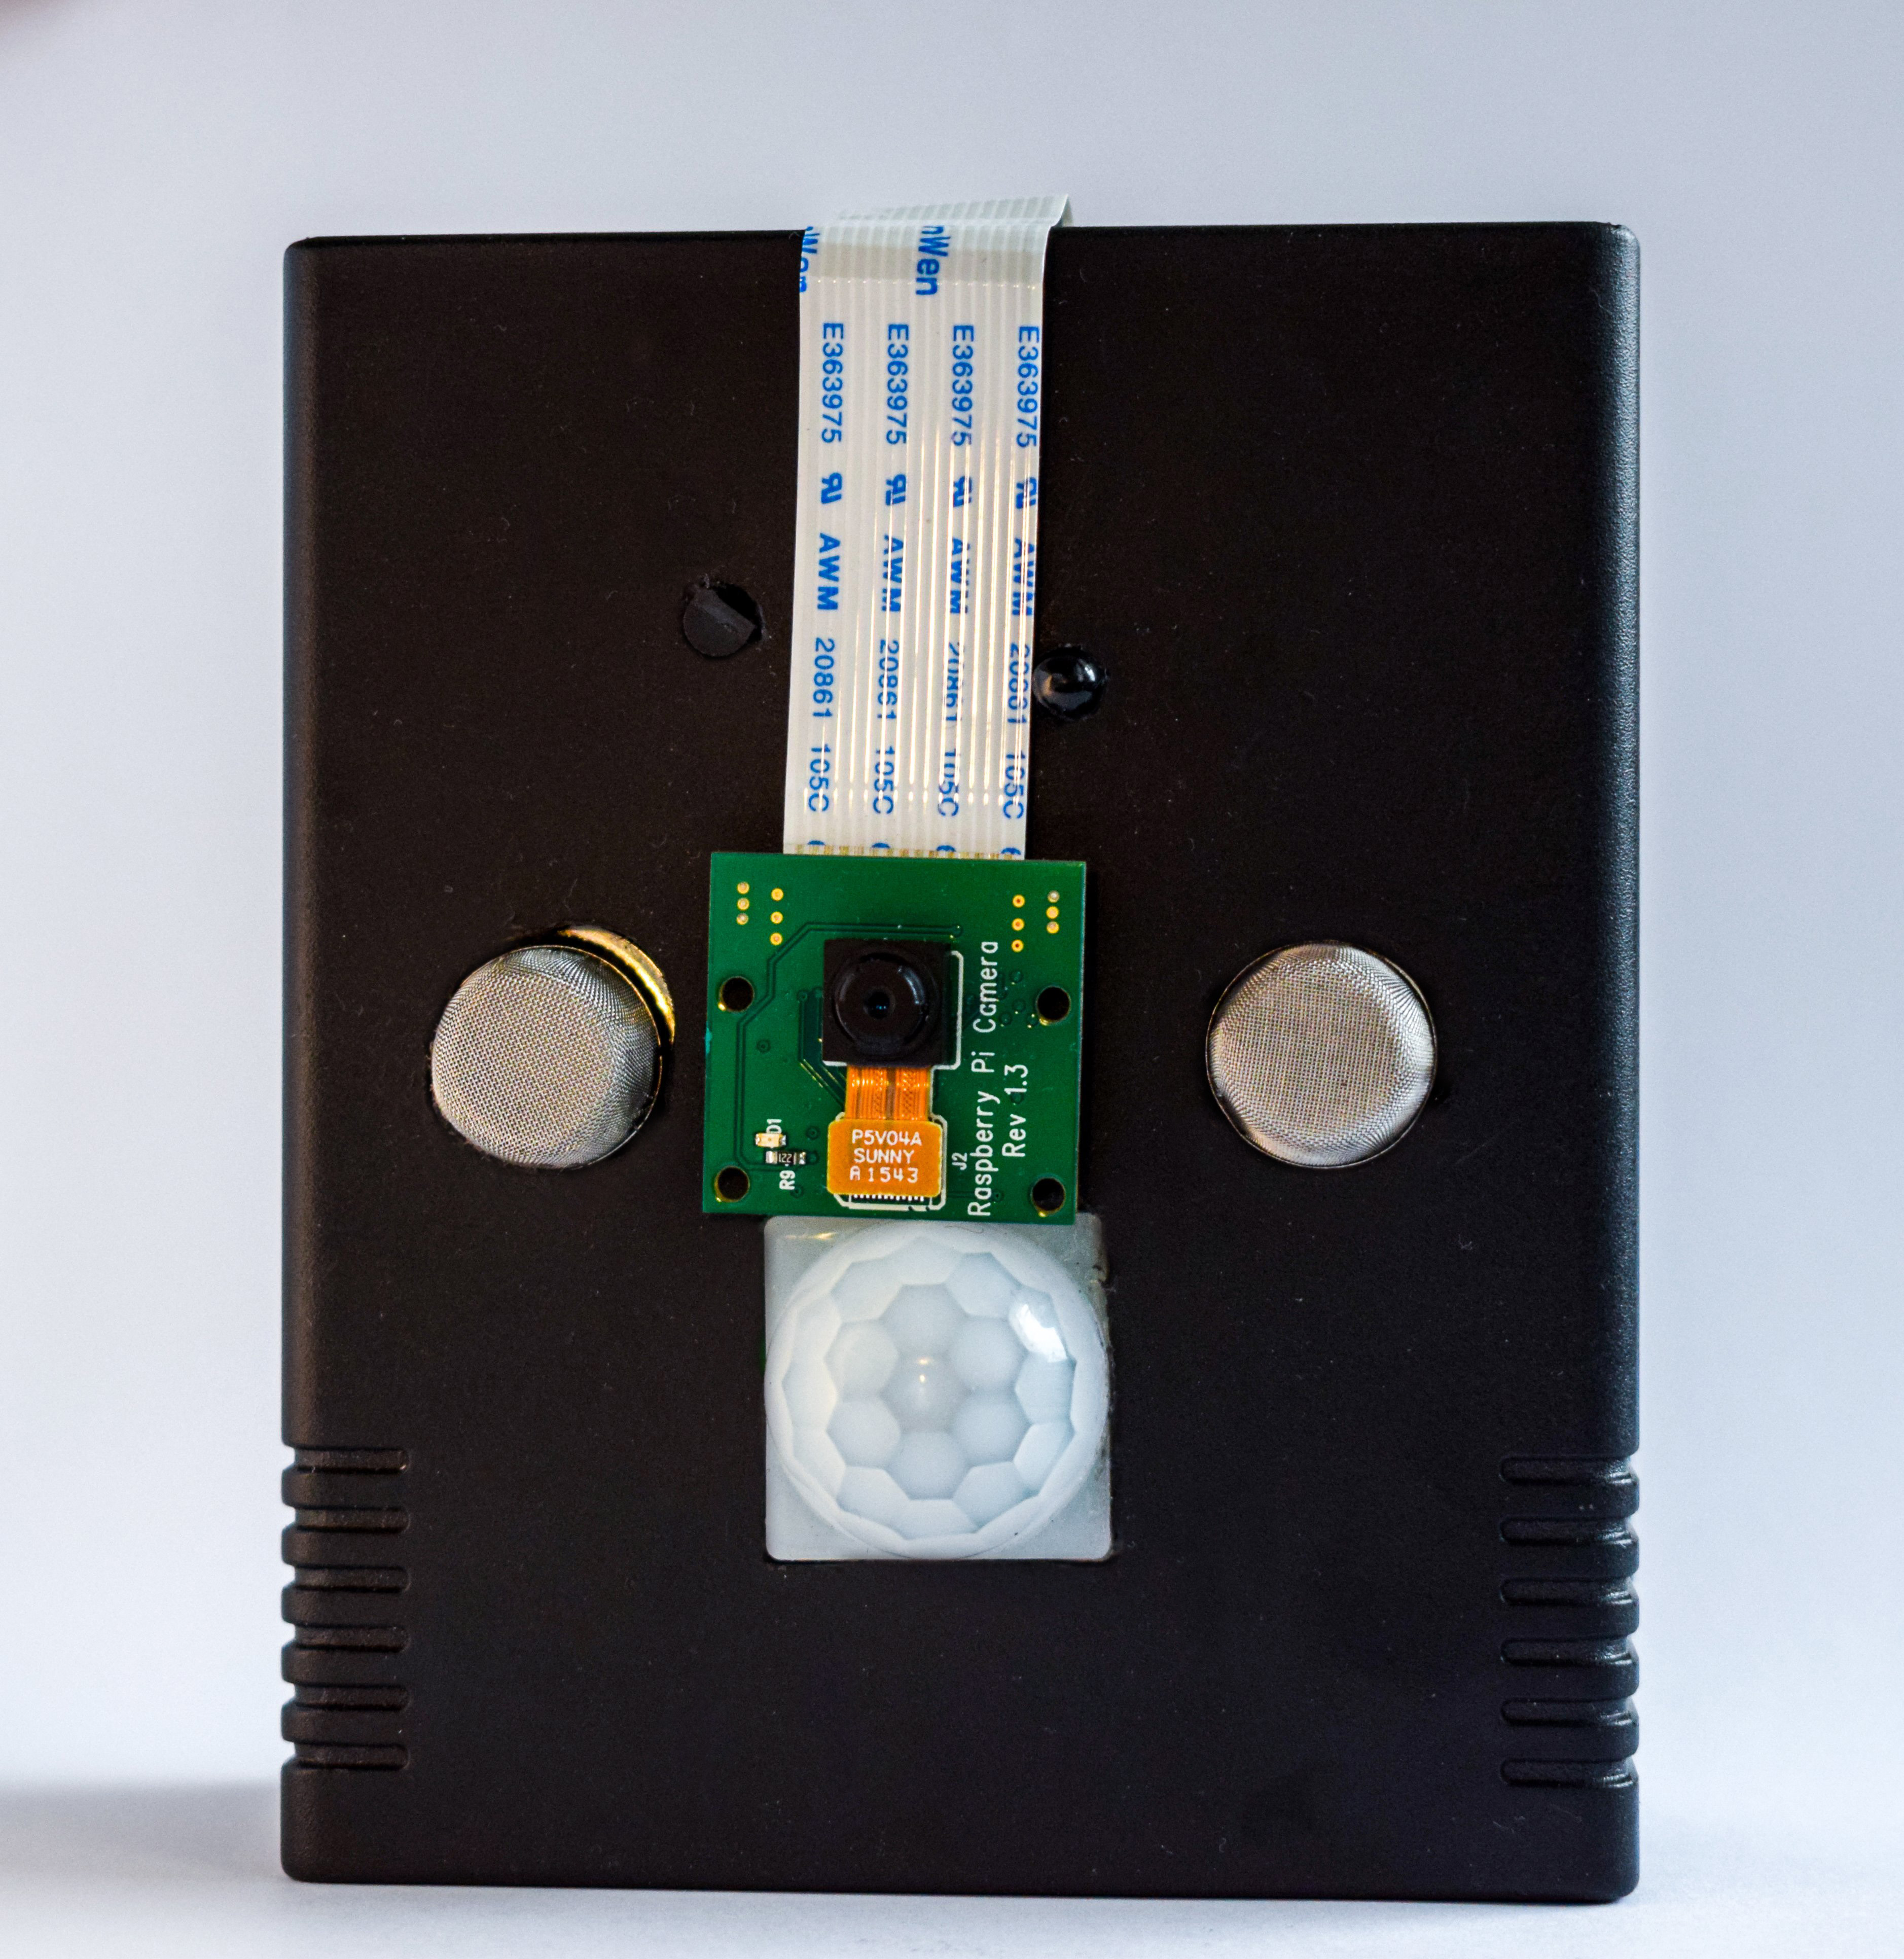
\includegraphics[width=7cm]{guard.jpg}
	\caption{Zbudowany zestaw The Guard [źródło własne]}
	\label{the_guard_set}
\end{figure}
\begin{figure}[h]
	\centering
	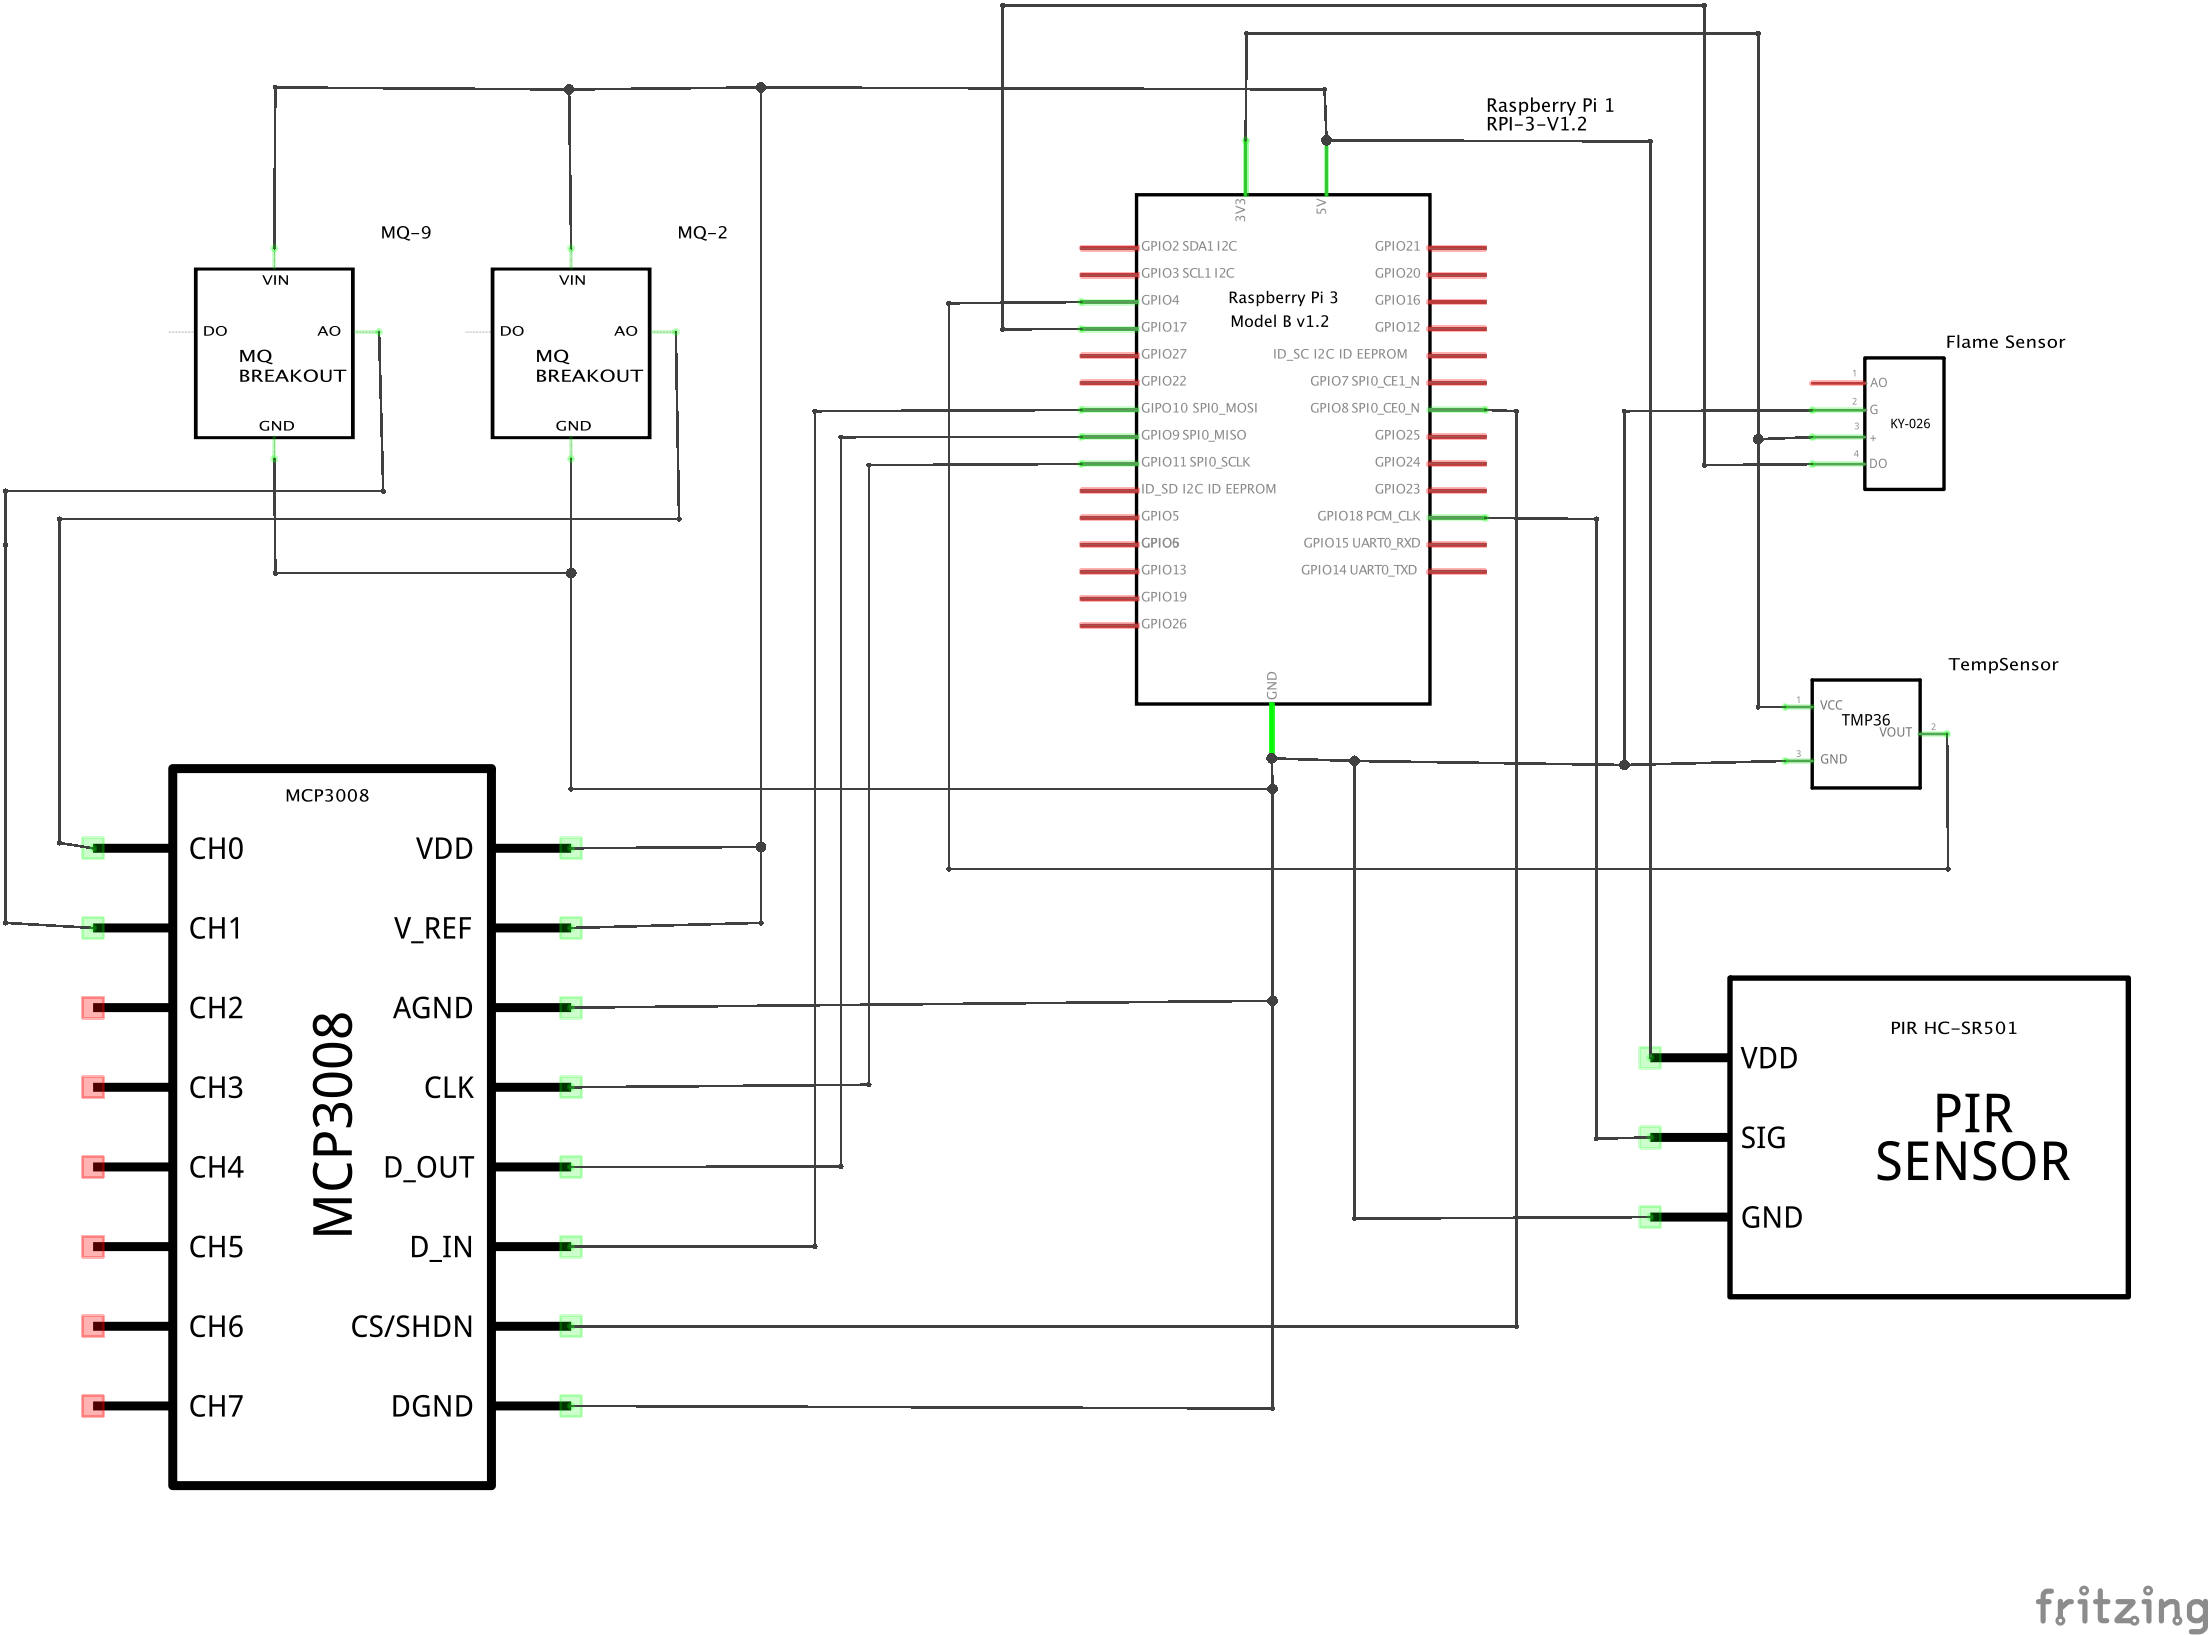
\includegraphics[width=15cm]{GuardSchem}
	\caption{Schemat układu The Guard [źródło własne]}
	\label{the_guard_schem}
\end{figure}
\paragraph{Specyfikacja Raspberry Pi 3:}
\begin{itemize} 
\item Procesor 1.2 GHz
\item Liczba rdzeni 4. Quad Core
\item Pamięć RAM 1 GB
\item Pamięć Karta microSD
\item 40 GPIO
\end{itemize}
Aby prawidłowo zainstalować oprogramowanie The Guard na dowolnym urządzeniu Raspberry Pi 3 należy wykonać poniższe czynności w terminalu:
\begin{enumerate} 
\item sudo apt-get install libx264-dev
\item cd /usr/src
\item git clone git://source.ffmpeg.org/ffmpeg.git
\item sudo ./configure --arch=armel --target-os=linux --enable-gpl --enable-libx264 --enable-nonfree
\item sudo make
\item sudo install
\item sudo nano /boot/config.txt
\item w pliku config.txt dopisać Dtoverlay=w1-gpio i Gpiopin=4
\item pip intall wiringpi
\item sudo pip install spidev
\item pip install pyrebase
\end{enumerate}
Następnym krokiem jest włączenie odpowiednich interfejsów w panelu konfiguracyjnym. Należy zmienić ustawienia zgodnie ze schematem (rys. \ref{rs_settings}).
\begin{figure}[ht]
	\centering
	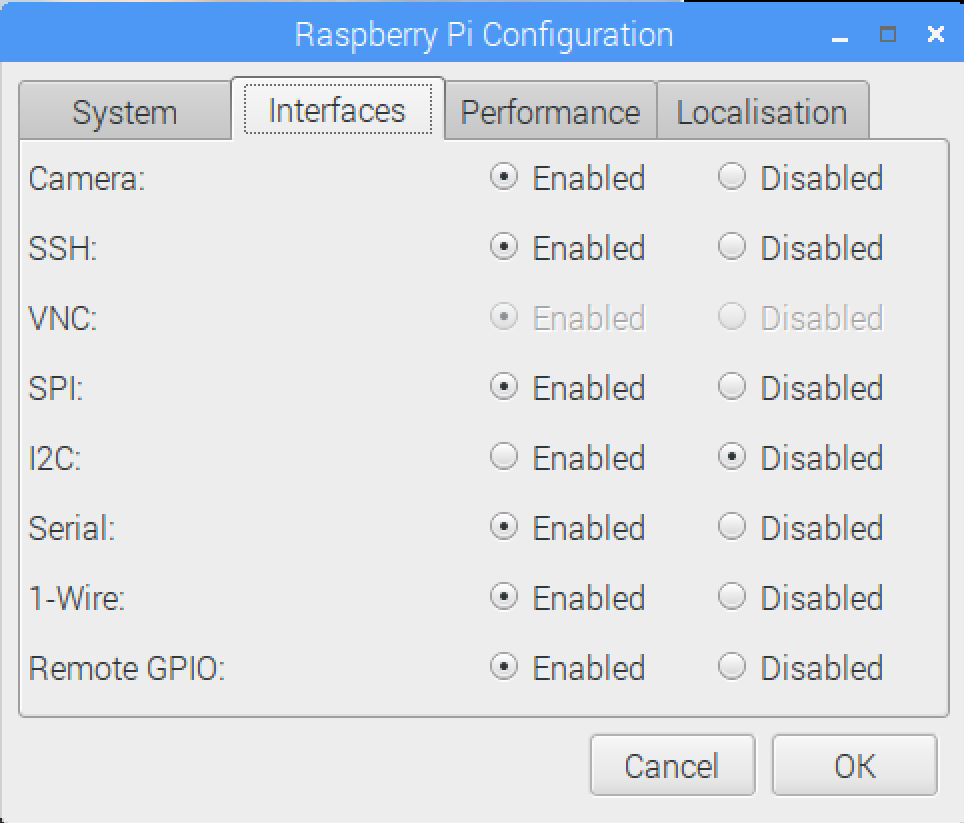
\includegraphics[width=6cm]{RSettings}
	\caption{Ustawienia [źródło własne]}
	\label{rs_settings}
\end{figure}
Użyto biblioteki wiringpi do odczytu danych z układów cyfrowych. Należy podkreślić, że numeracja fizycznych pinów(rys. \ref{gpio}) i numeracja pinów w wiringPi(rys. \ref{wiringpi}) jest różna i nie zawiera wszystkich dostępnych pinów na urządzeniu. Przykładowo odczyt pinu numer 1 w wiringPi jest równoznaczny z odczytem stanu na pinie numer 12 (GPIO18).
\begin{figure}[ht]
	\centering
	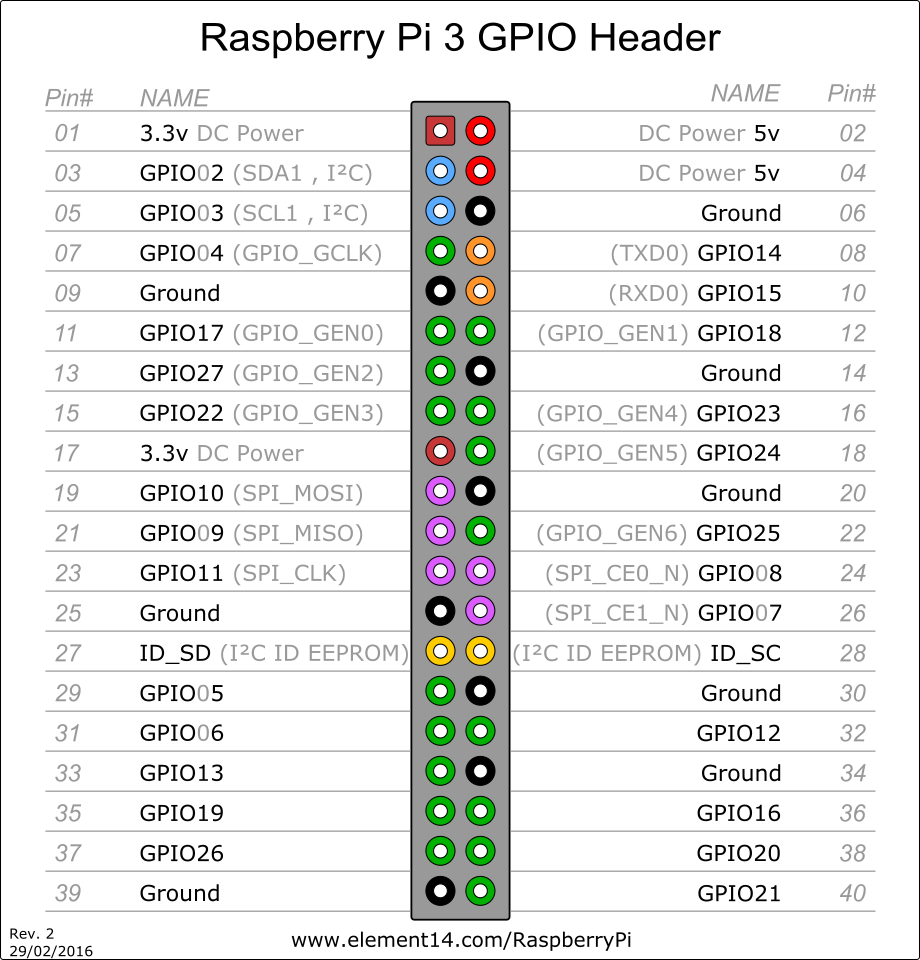
\includegraphics[width=6cm]{gpio.png}
        \caption{GPIO \cite{gpio}}
        \label{gpio}
\end{figure}
\begin{figure}[ht]
	\centering
	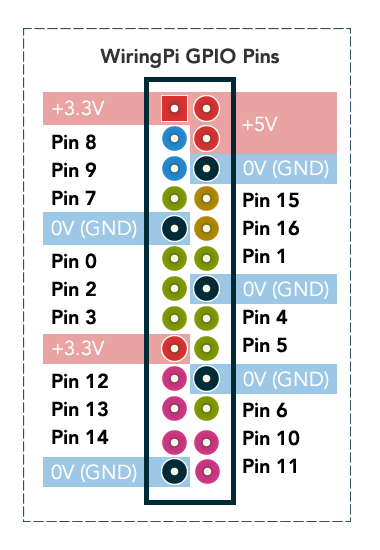
\includegraphics[width=4cm]{wiringpi.png}
        \caption{WiringPi \cite{wiringpi}}
        \label{wiringpi}
\end{figure}
Zainstalowane oprogramowanie odpowiedzialne jest za ciągłe monitorowanie stanów i zbieranie danych z czujników pomiarowych. Po podłączeniu układu do zasilania program jest uruchamiany automatycznie. Pierwszą czynnością jaką wykonuje Raspberry Pi jest wysłanie swojego numeru seryjnego do bazy danych Firebase. Cały proces jest w pełni zautomatyzowany. Dzięki temu użytkownicy od razu mogą dodać urządzenie i przeglądać dane z czujników na aplikacjach klienckich. Dodanie akcesorium pomiarowego następuje poprzez wprowadzenie w aplikacji jego numeru seryjnego.
\section{Czujniki}
Każdy zestaw składa się z 5 czujników analogowo cyfrowych,  jednej kamery i jednego przetwornika AC. 
\paragraph{a) Specyfikacja MQ-9 - czujnik tlenku węgla\cite{specyfikacjaMQ-9}:}
\begin{itemize} 
\item Zasilanie: 5 V
\item Pobór prądu: 150 mA
\item Temperatura pracy: od -10 do 50 \textdegree{}C
\item Wyjścia: analogowe oraz cyfrowe
\end{itemize}
\paragraph{b) Specyfikacja MQ-2 - czujnik LPG i dymu \protect\cite{specyfikacjaMQ-2}:}
\begin{itemize} 
\item Zasilanie: 5 V
\item Pobór prądu: 150 mA
\item Temperatura pracy: od -10 do 50 \textdegree{}C
\item Wyjścia: analogowe oraz cyfrowe
\end{itemize}
\paragraph{c) Specyfikacja czujnika wykrywania płomieni \protect\cite{specyfikacjaFlame}:}
\begin{itemize} 
\item Zasilanie: 3.3 V
\item Zakres wykrywanej fali: 760 do 1100nm
\item Kąt detekcji: od 0 do 60 stopni
\item Temperatura pracy: od -25 do 85 \textdegree{}C
\end{itemize}
\paragraph{d) Specyfikacja DS18B20 - czujnik temperatury \protect\cite{specyfikacjaTemp}:}
\begin{itemize} 
\item Zasilanie: 3.3 V
\item Zakres pomiarowy: od -55 do 125 \textdegree{}C
\end{itemize}
\paragraph{e) Kamera:}
\begin{itemize} 
\item Wykorzystano moduł kamery Raspberry Pi element14
\item Kamera 5MP - wspierająca nagrywanie 30 klatek na sekundę w rozdzielczości Full HD
\end{itemize}
\paragraph{f) Specyfikacja MCP3008 - przetwornik A/C \protect\cite{specyfikacjaAC}:}
\begin{itemize} 
\item Zasilanie: od 2.7V do 5.5V
\item Pobór prądu: 0.5 mA
\item Interfejs komunikacyjny: SPI
\item Liczba kanałów: 8
\item Rozdzielczość: 10bit
\end{itemize}
\paragraph{g) Specyfikacja czujnika ruchu PIR HC-SR501 \protect\cite{pir}:}
\begin{itemize} 
\item Zasilanie: od 4.5V do 20V
\item Pobór prądu w stanie czuwania: 50 uA
\item Zakres pomiarowy: maks. 7 m
\item Kąt widzenia: do 100\textdegree{}
\end{itemize}
Na schematach (rys. \ref{mq2}, rys. \ref{mq9}) przedstawiono charakterystykę czujników analogowych.
\begin{figure}[ht]
	\centering
	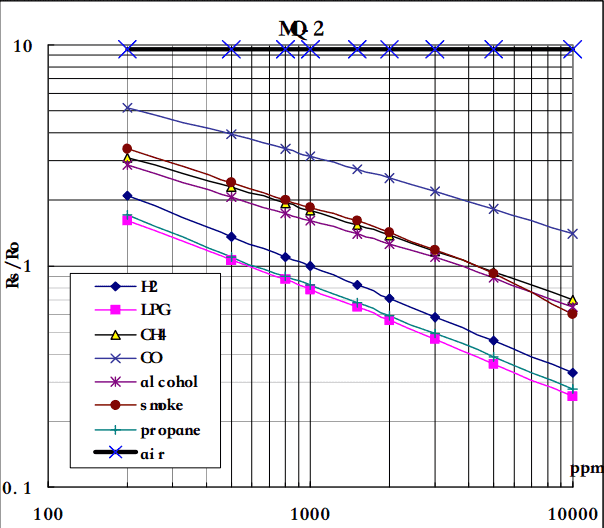
\includegraphics[width=8cm]{MQ2}
	\caption{Charakterystyka MQ-2 \protect\cite{mq2}}
	\label{mq2}
\end{figure}
\begin{figure}[ht]
	\centering
	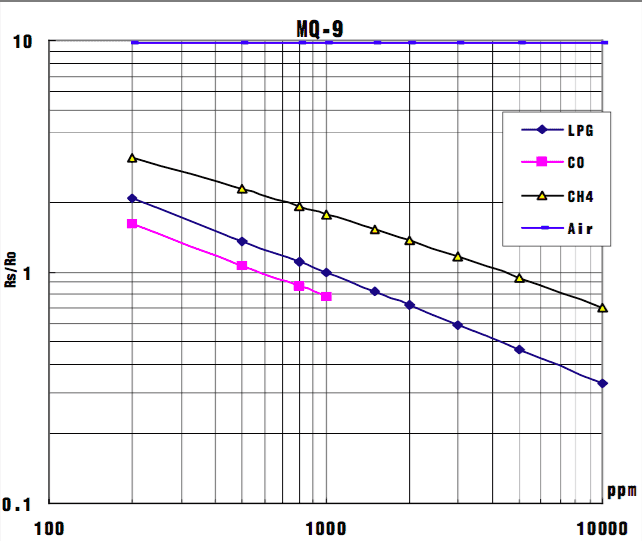
\includegraphics[width=8cm]{MQ9}
	\caption{Charakterystyka MQ-9 \protect\cite{mq9}}
	\label{mq9}
\end{figure}
Ro - jest to stała wartość oporu czujnika przy 1000ppm H2 w czystym powietrzu.\\
Rs - jest to opór czujnika w różnych stężeniach gazu.
Skoro Ro jest stałe to przy wzroście Rs czułość będzie maleć. Dlatego też im mniejszy stosunek Rs do Ro tym lepiej. Widać, że oba czujniki reagują na wiele różnych gazów. MQ-2 nazwano czujnikiem LPG a MQ-9 czujnikiem CO ze względu na to, że w stosunku do tych gazów mają najwyższą czułość. 

Niestety żaden model Raspberry nie posiada wbudowanego przetwornika analogowo cyfrowego dlatego konieczne było użycie układu zewnętrznego. Wybrano przetwornik MCP3008 ze względu na jego nisko koszt i interfejs SPI, który jest wspierany przez Raspberry Pi. MCP3008 to 10-bitowy przetwornik analogowy cyfrowy. Zasilany jest napięciem 5V.  Skoro jest to przetwornik 10-bitowy jest w stanie wykryć 1024 stany. Posiada 8 kanałów jednak w projekcie wykorzystano tylko 2 – dla MQ-9 i MQ-2.
\paragraph{Interfejs SPI:}
\begin{figure}[ht]
	\centering
	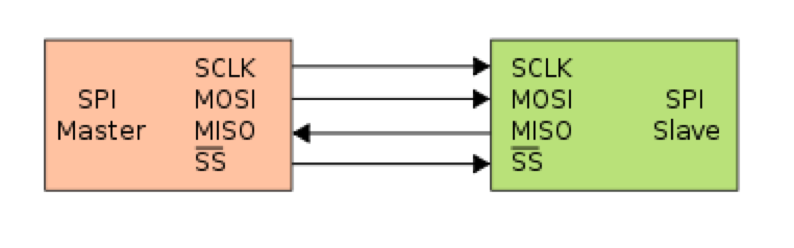
\includegraphics[width=5cm]{SPI.png}
	\caption{Interfejs SPI \protect\cite{spi}}
	\label{spi}
\end{figure}
SPI jest to interfejs synchroniczny(rys. \ref{spi}). Może być do niego podłączone wiele urządzeń typu slave, jednak tylko z jednym urządzeniem Master, które generuje zegar. Master poprzez linię SS wybiera urządzenie z którym chce się komunikować. \\
Interfejs ten zawiera jeszcze 3 linie:
\begin{enumerate} 
\item MOSI (ang. Master Output Slave Input): \\
Poprzez tę linię wysyłane są dane z Raspberry Pi do przetwornika analogowo cyfrowego MCP3008.
\item MISO (ang. Master Input Slave Output):\\
Poprzez tę linię wysyłane są dane z przetwornika AC do układu Master czyli w naszym przypadku Raspberry Pi 3
\item SCLK (ang. Serial Clock) :\\
Ta linia wykorzystywana jest do przesłania zegara wygenerowanego przez Rapberry Pi 3
\end{enumerate}
Do komunikacji poprzez ten interfejs wykorzystano bibliotekę spiDev. \\
Każdy układ monitoruje wskaźniki pomiarowe z czujników analogowych i cyfrowych. W przypadku wykrycia wskazań, które w znaczący sposób odbiegają od normy informuje właściciela o zagrożeniu. Informacja ta wysyłana jest do wszystkich urządzeń(smartfony, tablety itp), które posiada właściciel.  Analizując dane z czujników analogowych w czystym powietrzu, które wynoszą wtedy odpowiednio:\\
Czujnik MQ-9: od 0.15 do 0.2\\
Czujnik MQ-2: od 0.05 do 0.15\\
Przyjęto, że granicą wysłania notyfikacji do użytkownika jest przekroczenie progu 0.3. Wartości te to znormalizowane dane z przetwornika AC, który jak już wcześniej wspomniano wykrywa 1024 stany. Odczytywane wartości bezpośrednio na wyjściu przetwornika MCP3008 dla czujnika MQ-9 w czystym powietrzu to około 170. Stąd 170/1024 = 0.166. Wysłanie notyfikacji wiąże się z otrzymaniem wartości większej niż 308.
Czujniki cyfrowe wykorzystane w pracy informują o wykryciu płomieni i ruchu. Czujnik ruchu detekcję zagrożenia określa przez stan wysoki natomiast czujnik płomieni przez stan niski. W kodzie jednak wykonano instrukcje negacji, aby stan wysoki informował o niebezpieczeństwie a stan niski reprezentował jego brak. Na czujnikach znajduje się potencjometr, za pomocą którego dowolnie można ustawiać jego czułość. Odczyt danych następuje nieprzerwanie co 2 sekundy. Nie należy obawiać się, że czujnik ruchu nie wykryje zagrożenia z powodu braku odczytu we właściwym momencie, ponieważ utrzymuje on stan wysoki przez 5 sekund po wykryciu ruchu. Oprogramowanie wysyła także informacje z czujników do bazy danych Firebase. Zastosowanie takiej bazy daje możliwość monitorowania wszystkich danych w czasie rzeczywistym na aplikacjach klienckich. Dodatkowo w przypadku zagrożenia czyli przekroczeniu progu, o którym mowa wyżej wysyłana jest push notyfikacja do urządzeń użytkownika a informacja o zagrożeniu zapisywana jest w bazie danych Django. Każdy jest w stanie odtworzyć całą historię wydarzeń w swoim systemie.
Aby zapewnić wydajny i pewny system bezpieczeństwa przy otrzymaniu wysokich wartości na czujnikach zapisywany jest czas zdarzenia. Każda kolejna notyfikacja zostanie wysłana po upływie 10 minut od poprzedniej przy założeniu, że stan na czujniku nadal jest wysoki. 

\section{Obsługa wideo}

\paragraph{Protokół RTMP}
Podstawą funkcji strumieniowania wideo, jest protokół RTMP (Real-Time Message Protocol). Jest to, oparty na protokole TCP, protokół wysyłania obrazu, dźwięku oraz danych. \cite{MOBILERTMP}
Podstawową jednostką danych, w protokole RTMP, jest wiadomosć (ang. Message), której struktura jest zależna od typu strumieniowanych informacji. 
Wiadomosci dzielone są na kawałki (ang. Chunks), które są porcjami gotowymi do transmisji. Zatem strumień RTMP to ostatecznie strumień cząstek (ang. Chunk Stream) \cite{STREAMRTMP}

Ponadto, wykorzystano protokół HLS (HTTP Live Streaming), zapisywanie odbieranego obrazu, we wskazanej liczbie plików wideo o okreslonej dłusgoci. Gdy aplikacja kliencka odtwarza strumień wideo, w rzeczywistosci odbiera, strumieniowane po kolei, zapisane pliki ts. Wpływa to na opóźnienie odtwarzania, względem rzeczywistosci, z jednej strony, a z drugiej, dostarcza płynne wideo.

\paragraph{H264}
W pracy wykorzystano kodowanie obrazu koderem H.264. Charakteryzuje go niska złożonosć algorytmów kompresji oraz niewielkie opóźnienie, dzięki czemu idealnie nadaje się do zadania związanego z szybkim enkodowaniem obrazu, przed przestrumieniowaniem go dalej. \cite{H264}
Szybkoć i złożonoć H.264, idą w parze z jego jakoscią, która jest o wiele wyższa, niż w starszych rozwiązaniach.
Cechą charakterystyczną, dla tego typu kodowania wideo, jest użycie klatki kluczowej (ang keyframe, i-frame). Jest to pełna klatka obrazu, w przeciwieństwie, do następujących po niej danych, które wyrażają różnice między dwoma konsekutywnymi klatkami. Pozwala to na zmniejszenie rozmiarów, ostatecznego obrazu wideo.

\paragraph{Raspberry Pi}
Do obsługi strumieniowania wideo, po stronie Raspberry Pi, wykorzystywany jest program FFMPEG. Pozwala on na sterowanie strumieniem, od wyboru urządzenia wejsciowego, przez statystyki strumienia, po punkt docelowy. Dostęp do unikatowego, dla każdego urządzenia Raspberry, punktu końcowego, gwarantowało wczeniejsze pobranie nr seryjnego urządzenia. Poniżej przedstawiono skrypt, wykonujący wymienione funkcje \cite{raspivid}:
\begin{verbatim}
#!/bin/bash
serial_id="$(cat /proc/cpuinfo | grep Serial | cut -d ' ' -f 2)"
raspivid -o - -t 0 -fps 30 -b 1000000 | ffmpeg -re -ar 44100 -ac 2 
-acodec pcm_s16le -f s16le -i /dev/zero -f h264 -i - -vcodec copy -g 60 
-strict experimental 
-f flv rtmp://52.236.165.15:1936/camera/${serial_id}
\end{verbatim}
Pierwszą czynnoscią, wykonywaną w skrypcie, jest otwarcie pliku /proc/cpuinfo, następnie znajdowana jest w nim linia, w której znajduje się wyjątkowy serial urządzenia. Na końcu, z wykorzystaniem potoku, i funkcji cut, wartosć ta zostaje przypisana do zmiennej serialid.

W drugiej linii skryptu wykorzystane jest narzędzie linii poleceń Raspberry - raspivid. Pozwala ono pobrać obraz z kamery. 
\begin{itemize}
\item Pierwszym przełącznikiem jest -o z parametrem -. Oznacza to, że obraz z kamery jest wysyłany na wyjscie standardowe.
\item Przełącznik -t ustawiony na 0 pozwala przekazywać obraz, z modułu kamery, przez nieokrelony czas. Aby przestać pobierać wideo, należy użyć przerwania za pomocą sygnału SIGINT (obsługiwanego w terminalu skrótem klawiszowym CTRL+C).
\item Opcja -fps pozwala wskazać liczbę przechwytywanych klatek w ciągu sekundy. Tutaj wykorzystano maksymalne możliwoci wybranego modułu kamery.
\item Ostatnią opcją, wykorzystaną w pobieraniu obrazu z kamery, jest bitrate, tzn wielkosć pamięci, w której ma się znaleźć obraz przechwycony w ciągu 1 sekundy. Ustawienie opcji -b na 1000000 oznacza, że 1 sekunda wideo, może zajmować 125 kilobajtów pamięci. Jest to szczególnie istotna informacja, w kontekcie transmisji obrazu poza urządzenie.
\end{itemize}

Drugim poleceniem jest wywołanie narzędzia ffmpeg, połączonego za pomocą potoku, odbierającego, przechwytywany za pomocą funkcji raspivid, obraz i przekazującego go na docelowy punkt końcowy. Za jego pomocą ustala się ostatecznie opcje kodujące obraz i dźwięk w trakcie końcowej transmisji.
\begin{itemize}
\item Przełącznik -re pozwala odczytywać dane wejsciowe, z oryginalną częstotliwoscią. Zatem zostają przechwycone ustawienia przełącznika funkcji raspivid -fps 30.
\item Opcje  -ar, -ac, -acodec, -f, -strict odpowiadają kolejno za: próbkowanie dźwięku, wybór liczby kanałów, kodek audio, format dźwięku oraz wybór eksperymentalnego sposobu kodowania. Wymuszenie wykorzystania, jako wejscia strumienia dźwięku, na /dev/zero, oznacza, że strumień ten zostaje wypełniony wartosciami pustymi. Zatem opcje transmisji dźwięku są nieistotne.
\item Przełącznik -vcodec ustala kodek wideo. W pracy wykorzystano standard kodowania h264.
\item Następnie ustawiono wejscie obrazu. Przełącznik -i - powoduje, że narzędzie ffmpeg przechwytuje, dzięki potokowi, obraz przekazywany funkcją raspivid.
\item Opcja -g 60 oznacza, że tzw klatka kluczowa (ang keyframe) pojawia się co 60 klatek. W tej sytuacji, co 2 sekundy. 
\item Przełącznik -f, w przypadku strumienia obrazu z kamery, wymusza format nadawanego wideo.  
\item Ostatnim elementem polecenia jest podanie punktu docelowego dla strumienia. Za pomocą protokołu RTMP, obługiwanego przez serwer o adresie IP 52.236.165.15 na porcie 1936, obraz wysyłany jest na aplikację o nazwie camera i punkt charakteryzowany przez serial urządzenia. Działanie tego elementu opisano w kolejnym punkcie. 
\end{itemize}

\paragraph{Serwer}
Narzędziem, umożliwiającym obsługę strumieniowania wideo, z wielu źródeł, na wiele urządzeń równoczesnie, jest serwer NGINX. W częsci projektu, związanej ze strumieniowaniem wideo, wykorzystano moduł nginx-rtmp \cite{NGINX}. 
Moduł ten pozwala, m. in., na:
\begin{itemize}
\item Tworzenie dynamicznych punktów końcowych, dla urządzeń strumienujących obraz
\item Zmianę parametrów przechwytywanego obrazu 
\item Zapisywanie nagrań po stronie serwera
\item Tworzenie punktów nadających, dla aplikacji odtwarzających strumień
\end{itemize}
Ponadto pozwala na utworzenie aplikacji HLS, przechowującej tymczasowo obraz, zanim zostanie on przestrumieniowany dalej. Pozwala to na uniknięcie opóźnień między kolejnymi klatkami obrazu.

Wszystkie funkcjonalnosci definiują poniższe ustawienia pliku konfiguracyjnego, którego lokalizacja to /usr/local/nginx/conf/nginx.conf:

\begin{verbatim}
rtmp {
    server {
            listen 1936;
            chunk_size 4096;
            application camera {
                    hls on;
                    hls_path /mnt/hls/;
                    hls_fragment 2;
                    hls_playlist_length 3;
                    allow publish all;
                    allow play all;
                    live on;
                    record off;
             }
    }
}
\end{verbatim}

Powyższe linie powodują, że serwer rtmp, dostępny jest na porcie 1936 (domyslne porty dla protokołu RTMP, na urządzeniu z systemem z rodziny Ubuntu,  to 1935 i 1936). Następnie tworzona jest aplikacja o nazwie camera. Dla aplikacji strumieniujących dane, jest ona dostępna pod adresem: rtmp://<ip-serwera>:1936/camera/<klucz>, gdzie klucz jest wybierany przez aplikację strumieniującą i tworzony dynamicznie, gdy tylko urządzenie zacznie nadawać dane pod wskazany adres.
Ustawienia aplikacji decydują o tym, że dla urządzeń odtwarzających wideo, dostępne jest ono dzięki aplikacji HLS - opcja hls on. Na szczególną uwagę zasługują linie: hls fragment 2 oraz hls playlist length 3, które wskazują na to, że po stronie serwera, nagrywane będą 2 tymczasowe fragmenty, o długoci 3 sekund, każdy. Pliki te będą przechowywane w folderze /mnt/hls/, a ich nazwę jednoznacznie będzie wskazywać klucz strumienia.

\begin{verbatim}
http {
    server {
        listen       80;
        location /hls {
                types {
                        application/vnd.apple.mpegurl m3u8;
                        video/mp2t ts;
                }
        root /mnt/;
        }
    }
}
\end{verbatim}

Konfiguracja ta udostępnia aplikację HLS. Dla aplikacji klienckich, obraz będzie dostępny pod adresem: http://<ip-serwera>:80/hls/<klucz>.m3u8, o czym decyduje konfiguracja częsci związanej z serwerem RTMP.

Wykorzystane funkcjonalnosci narzędzia Nginx nie wykorzystują w pełni możliwosci produktu, jednak projekt nie wymagał korzystania z funkcji serwera proxy.
